%****************************** Preambulo ******************************%
\documentclass[letterpaper, 12pt]{article}

% El paquete selecciona el idioma de trabajo. En las opciones se tiene el cambio del inglés al español, traduce "table" a "tabla" y el cambio de la coma por el punto decimal, en ese orden.
\usepackage[spanish, es-tabla, es-nodecimaldot]{babel}

% Paquete que soluciona los problemas de acentos y la inserción de la ñ.
\usepackage[utf8]{inputenc}

% Paquete necesario para insertar imágenes.
\usepackage{graphicx}

% Paquete que corrige la ubicación de imágenes. \begin{figure}[H]
\usepackage{float}

%Añade comandos útiles como para notación de unidades y simplifica el código para derivadas. El amsmath añade otros entornor matemáticos.
\usepackage{physics, amsmath}

% Este paquete sirve para modificar el estilo de la página. Aunque tiene opciones, YO las voy a modificar más adelante en el documento y por eso no las defino en este punto (para evitar posibles errores). ~~J
\usepackage{geometry}

% Permite bloques de texto literal que pueden continuar de una página a otra.
\usepackage{fancyvrb}
\DefineVerbatimEnvironment{PromptBlock}{Verbatim}{fontsize=\footnotesize, xleftmargin=0.05\textwidth}

% Mejora la legibilidad separando visualmente los párrafos y manteniendo una sangría clara.
\setlength{\parskip}{0.75em}
\setlength{\parindent}{0em}

% Permite crear gráficos estilizados y de alta calidad con el lenguaje nativo de latex.
\usepackage{tikz}
\usetikzlibrary{fit, backgrounds, arrows.meta}
    
% Determina el tamaño de separación entre columnas
\usepackage{multicol}
\setlength\columnsep{20pt}

% A lo largo del texto habrá cosas que enumerar y enumitem es mucho mejor que simplemente enumerate.
\usepackage{enumitem}

% Se usa principalmente en ejercicios resueltos para ahorrar espacio.
\usepackage{relsize}
\newcommand{\mlr}[1]{\mbox{$\mathlarger{#1}$}}

% Escribe las unidades
\newcommand{\un}[1]{\mbox{ #1}}

% Permite escribir las citas arribita UwUr
\newcommand{\upcite}[1]{\mbox{$^\text{\cite{#1}}$}}

% Agrega enlaces internos de las secciones, figuras y tablas. "hypersetup" da color a los enlaces dentro del documento.
\usepackage{hyperref}
\hypersetup{
  colorlinks = true,
  linkcolor = blue,
  filecolor = magenta,
  urlcolor = cyan,
  citecolor = red
}

%****************************** Documento ******************************%
\begin{document}
   
    \newgeometry{hmargin=2cm, vmargin=2cm}
    
    %~~~~~~~~~~~~~~~~~~~~~~~~~~~~~~~~~~~~~~~~~~~~~~~~~~~~~~~~~~~~~~~~~~~~~~~~~~%
    % Esta parte corresponde al título y el resúmen, no borrar. ~~J
    
    % Aquí comienza el documento y por lo tanto la numeración de las páginas; este comando indica que a partir de este punto las páginas tendrán numeración y que estará en números romanos.
    \pagenumbering{Roman}
    
    \begin{center}
        {\huge\bfseries Emulador de los \emph{kernels} $F_2$ y $G_2$ en gravedad modificada.}
        
        \vspace{2.5em}
        
        {\large Jair Ferrara Andrade}
    \end{center}
    
    \vspace{0.5em}
    
    \begin{abstract}
         
         Se presenta un emulador para calcular los \emph{kernels} de segundo orden $F_2$ y $G_2$ en modelos de gravedad modificada tipo Hu-Sawicki con $n = 1$. A partir de la teoría de perturbaciones, el problema se formula en términos de las funciones $\mathcal{A}$ y $\mathcal{B}$, que contienen algunas de las correcciones no lineales, en particular las que incluyen los efectos de apantallamiento. Para aproximar estas cantidades, se genera un conjunto de datos mediante la resolución numérica de las ecuaciones diferenciales correspondientes y se entrena una red neuronal MLP, cuyas entradas son parámetros cosmológicos y configuraciones de momento. El emulador reproduce adecuadamente el comportamiento de $\mathcal{A}$ y $\mathcal{B}$ y permite obtener los \emph{kernels} con tiempos de ejecución del orden de milisegundos. Aunque las derivadas presentan errores relativos mayores que las funciones principales, el modelo captura su tendencia general.
         
    \end{abstract}
    
    \vspace{1.5em}
    
    %~~~~~~~~~~~~~~~~~~~~~~~~~~~~~~~~~~~~~~~~~~~~~~~~~~~~~~~~~~~~~~~~~~~~~~~~~~%
    % Esta parte no se borra, es el índice. ~~J  ¿A que sí se borra? uwu --C
    \noindent\rule{\textwidth}{1pt}
    
    \tableofcontents	% Genera una tabla de contenido o índice.
    
    \vspace{1em}
    
    \noindent\rule{\textwidth}{1pt}
    %~~~~~~~~~~~~~~~~~~~~~~~~~~~~~~~~~~~~~~~~~~~~~~~~~~~~~~~~~~~~~~~~~~~~~~~~~~%
    
    \vspace*{1.5em}
    %\newpage
    
    % Aquí inicia el entorno de multicol. Si se quieren insertar imágenes, simplemente hay que terminar el entorno, insertar la imagen y abrir otro entorno. ~~J

    \section{Teoría}
        \subsection{Breve repaso de teoría de perturbaciones}
            La teoría de perturbaciones parte de una idea sencilla: aunque el universo es estadísticamente homogéneo a grandes escalas, localmente aparecen sobredensidades de materia que contienen información cosmológica. Para cuantificar esas desviaciones se introduce el contraste de densidad
            
            \begin{equation}
                \delta(\vb{x},t) = \frac{\rho(\vb{x},t) - \bar{\rho}(t)}{\bar{\rho}(t)}.
            \end{equation} 
            
            En esta expresión, $\rho(\vb{x},t)$ es la densidad de materia y $\bar{\rho}(t)$ la densidad de materia de fondo. Para seguir su evolución, conviene pasar al espacio de Fourier, donde las derivadas reducen su complejidad al reducirse a factores algebraicos. En el régimen lineal, cuando $\delta \ll 1$, cada modo crece de manera independiente y se puede escribir como $\delta(\vb{k},t) = D_+(t)\delta_0(\vb{k})$. El factor $D_+(t)$ resume ese crecimiento y satisface:
            
            \begin{equation}\label{eq:factor_de_crecimiento}
                \hat{\mathcal{T}}D_+ = 4\pi G\bar{\rho}D_+.
            \end{equation}
            
            El operador que aparece en esta ecuación se define, usando $H$ para denotar el parámetro de Hubble, como
            
            \begin{equation}
                \hat{\mathcal{T}} = \dv[2]{}{t} + 2H\dv{}{t}.
            \end{equation}

            Esta es la aproximación lineal y se puede mejora al considerar términos no lineales de la expansión de las sobredensidades de materia y velocidad:
            
            \begin{align}
                \delta(\vb{k},t) = \sum_{n = 1}^\infty \delta^{(n)}(\vb{k},t), \\
                \theta(\vb{k},t) = \sum_{n = 1}^\infty \theta^{(n)}(\vb{k},t).
            \end{align}

            En teoría de perturbaciones estándar, los términos de orden $n$ se escriben como convoluciones de $n$ sobredensidades lineales pesadas por los \emph{kernels} $F_n$ y $G_n$:
            
            \begin{align}
                \delta^{(n)}(\vb{k}) = 
                (2\pi)^3 \int_{\vb{k}_{1\cdots n}} F_n(\vb{k}_1,\ldots,\vb{k}_n) 
                \delta_D\qty(\vb{k}-\vb{k}_{1\cdots n}) \prod_{i=1}^{n}\delta_0(\vb{k}_i), \\
                \theta^{(n)}(\vb{k}) = 
                (2\pi)^3 \int_{\vb{k}_{1\cdots n}} G_n(\vb{k}_1,\ldots,\vb{k}_n) 
                \delta_D\qty(\vb{k}-\vb{k}_{1\cdots n}) \prod_{i=1}^{n}\delta_0(\vb{k}_i),
            \end{align}
            
            donde $\vb{k}_{1\cdots n} = \vb{k}_1 + \cdots + \vb{k}_n$ y $\int_{\vb{k}} \equiv \int\dd^3k/(2\pi)^3$.

            El observable más común asociado a la sobredensidad es el espectro de potencias $P(k)$ y se define como

            \begin{equation}
                \expval{\delta(\vb{k})\delta(\vb{k}')}=(2\pi)^3\delta_D(\vb{k}+\vb{k}')P(k).
            \end{equation}

            El espectro de potencias lineal se encuentra con el primer orden del desarrollo de la sobredensidad. Las primeras correcciones son las llamadas 1-\emph{loop}, $P_\text{1-loop}(k) = P_L(k) + P_{22}(k) + P_{13}(k)$, donde aparece la necesidad de conocer los \emph{kernels}:

            
            \begin{align}
                P_{22}(k) &= 2\int_{\vb{q}} \qty[F_2(\vb{q},\vb{k}-\vb{q})]^2 P_{\mathrm{L}}(q)P_{\mathrm{L}}(\abs{\vb{k}-\vb{q}}), \\
                P_{13}(k) &= 6P_{\mathrm{L}}(k)\int_{\vb{q}} F_3(\vb{k},\vb{q},-\vb{q})P_{\mathrm{L}}(q).
            \end{align}
            
        \subsection{\texorpdfstring{Los \emph{kernels} $F_2$ y $G_2$ en teoría de gravedad modificada}{Los kernels F2 y G2 en teoría de gravedad modificada}}
            Los modelos de gravedad modificada $f(R)$ consisten en cambiar la acción de Hilbert-Einstein reemplazando el escalar de Ricci por una función de este. Una de sus consecuencias se puede manifestar como modificaciones a la gravedad newtoniana. El modelo general se puede representar mediante la ecuación de Poisson correspondiente, en el espacio de Fourier:

            
            \begin{equation}
                -\frac{k^2}{a^2}\Phi(\vb{k}) = 4\pi G\bar{\rho}\mu(k,t)\delta(\vb{k}) + S(\vb{k}),
            \end{equation}
            
            con los términos $\mu(k,t)$ y $S(\vb{k})$ siendo dependientes del modelo de gravedad que se esté estudiando. Al introducirlos en la expresión lineal, la ecuación de crecimiento \ref{eq:factor_de_crecimiento} se modifica de la siguiente manera:
            
            \begin{equation}\label{eq:crecimiento_no-lineal}
                \hat{\mathcal{T}}D_+ = 4\pi G\bar{\rho}\mu(k,t)D_+ = A(k,t)D_+.
            \end{equation}

            Como el crecimiento lineal entra en la construcción de la teoría de perturbaciones, cualquier cambio en $D_+$ se propaga a las sobredensidades de orden superior. En consecuencia, también cambian las expresiones de los \emph{kernels}. Para este caso, las formas relevantes son \cite{1}:
            
            \begin{align}
                F_2(\vb{k}_1,\vb{k}_2) &= \frac12 + \frac{3}{14}\mathcal{A}
                + \qty(\frac{1}{2}-\frac{3}{14}\mathcal{B})\frac{(\vb{k}_1\cdot \vb{k}_2)^2}{k_1^2k_2^{2}}
                + \frac{\vb{k}_1\cdot \vb{k}_2}{2k_1^2 k_2^2}\qty(\frac{k_1}{k_2}+\frac{k_2}{k_1}), \\ 
                G_2(\vb{k}_1,\vb{k}_2) &=\frac{3\mathcal{A}(f_1+f_2)+3\dot{\mathcal{A}}/H}{14f_0}
                + \qty(\frac{f_1+f_2}{2f_0}-\frac{3\mathcal{B}(f_1+f_2)+3\dot{\mathcal{B}}/H}{14f_0})\frac{(\vb{k}_1 \cdot \vb{k_2})^2}{k_1^2k_2^2} \nonumber\\
                & + \frac{\vb{k}_1\cdot \vb{k}_2}{2k_1k_2}\qty(\frac{f_2 k_2}{f_0 k_1}-\frac{f_1 k_1}{f_0 k_2}),
            \end{align}
            
            donde se introduce la tasa de crecimiento de cada modo y la ecuación que satiface $f_0$
            
            \begin{equation}
                f_i(k_i,t) = \dv{\log D_+(k_i,t)}{\log a(t)}
            \end{equation}
            
            Las funciones $\mathcal{A}$ y $\mathcal{B}$ concentran entonces la información de segundo orden. En términos del factor de crecimiento se escriben como
            
            \begin{equation}
                \mathcal{A}(\vb{k}_1,\vb{k}_2,t) = \frac{7D^{(2)}_\mathcal{A} (\vb{k}_1,\vb{k}_2,t)}{3D_+(k_1,t)D_-(k_2,t)} \qq{y} 
                \mathcal{B}(\vb{k}_1,\vb{k}_2,t) = \frac{7D^{(2)}_\mathcal{B} (\vb{k}_1,\vb{k}_2,t)}{3D_+(k_1,t)D_-(k_2,t)}
            \end{equation}
            
            El problema queda reducido a encontrar $D_\mathcal{A}^{(2)}$ y $D_\mathcal{B}^{(2)}$. Estas cantidades no se fijan algebraicamente, sino como soluciones de las siguientes ecuaciones diferenciales \cite{2}:
            
            \begin{align}
                \qty(\hat{\mathcal{T}} - A(k))D_\mathcal{A}^{(2)} 
                &= \qty[ A(k) 
                + (A(k) - A(k_1))\frac{\vb{k}_1 \cdot \vb{k}_2}{k_2^2} 
                + (A(k) - A(k_2)) \frac{\vb{k}_1 \cdot \vb{k}_2}{k_1^2} 
                + \mathcal{S}^{(2)}(\vb{k}_1, \vb{k}_2) ] \nonumber\\
                & \qq{} \times D_+(k_1) D_+(k_2), \label{eq:DA}\\
                \qty(\hat{\mathcal{T}} - A(k))D_\mathcal{B}^{(2)} &= \Big[ A(k_1) + A(k_2) - A(k) \Big] D_+(k_1)D_+(k_2), \label{eq:DB}
            \end{align}
            
            y la definición de las fuentes no lineales, el término $\mathcal{S}(\vb{k})$ se expande como
            
            \begin{equation}
                S(\vb{k}) = \frac{1}{2} \int_{\vb{k}_{12}} \mathcal{S}^{(2)}(\vb{k}_{1},\vb{k}_{2}) \delta(\vb{k}_{1}) \delta(\vb{k}_{2}) dk_{2} + \frac{1}{6} \int_{\vb{k}_{123}} \mathcal{S}^{(3)}(\vb{k}_{1},\vb{k}_{2},\vb{k}_{3}) \delta(\vb{k}_{1}) \delta(\vb{k}_{2}) \delta(\vb{k}_{3}) + \dots
            \end{equation}
        
        \subsection{\texorpdfstring{El sistema que rige las funciones $\mathcal{A}$ y $\mathcal{B}$}{El sistema que rige las funciones A y B}} 

        En este trabajo se considera el caso particular de los modelos de Hu-Sawicki con $n = 1$. Los detalles específicos se pueden encontrar en el apéndice B de \cite{1}. Para encontrar los valores de $\mathcal{A}$ y $\mathcal{B}$, primero hay que resolver las ecuaciones diferenciales \ref{eq:DA} y \ref{eq:DB}. Por ahora, la tarea que se debe hacer es encontrar una forma que solo depende de los parámetros cosmológicos.

        El primer paso es usar tiempo conforme para trabajar con un sistema más conveniente. Se toma $\eta = -\log(1 + z)$ y, bajo esta transformación, el operador $\hat{\mathcal{T}}$ toma la forma
        
        \begin{equation}\label{eq:operador_conforme}
            \hat{\mathcal{T}} = H^2(\eta)\qty[\dv[2]{}{\eta} + f_1(\eta)\dv{}{\eta}],
        \end{equation}
        
        siendo las las abreviaturas y la ecuación que satisface $f_0$
        
        \begin{equation}
            f_1(\eta) = 2 - \frac32\Omega_m(\eta) \qc f_2(\eta) = \frac32\Omega_m(\eta) \qq{y} f_0^{\prime}(\eta) = f_2(\eta) + f_0(\eta)^2 - f_1(\eta)f_0(\eta).
        \end{equation}
        
        La misma transformación también permite expresar el término gravitacional efectivo como
        
        \begin{equation}\label{eq:termino_A}
            A(k,t) = A_0\,\mu(k,t), \qquad A_0=4\pi G\bar\rho=\frac{3}{2}\Omega_m(\eta)\,H^2(\eta),
        \end{equation}
        
        donde se usó $\bar\rho=\Omega_m\,3H^2/(8\pi G)$, y, para completar la dependencia temporal, se emplean
        
        \begin{equation}
            \Omega_m(\eta) = \qty(1+\frac{1-\Omega_{m0}}{\Omega_{m0}}e^{3\eta})^{-1}, \qq{}
            H(\eta) = H_0\sqrt{\Omega_{m0} e^{-3\eta}+(1-\Omega_{m0})}, \\
        \end{equation}
        
        donde $\Omega_{m0} = \Omega_{m}(\eta = 0)$ representa el valor presente de la densidad de materia.

        Es hasta aquí donde nos detenemos para utilizar el ejemplo del modelo HS, en particular, porque los término $\mu(k,\eta)$ y $\mathcal{S}(\vb{k})$ dependen del modelo. En este caso, la modificación a la acción es:
        
        \begin{equation}
            f(R) = -\frac{\Omega_{m0}}{6(1 - \Omega_{m0})} \frac{R}{R/M^2 + 1},
        \end{equation}
        
        con $M = H_0^2\Omega_{m0}$. De esta elección se siguen las expresiones
        
        \begin{equation}
            \mu(\eta,k) = 1+\frac13\,\frac{k^2}{k^2+e^{2\eta}m^2(\eta)} \qq{y} 
            \mathcal{S}^{(2)}(k_1,k_2) 
            = -\qty(\frac{2\mathcal{A}_0}{3})^{2} \frac{M_2(k_1,k_2)\,k^2/a^2}{6\,\Pi(k_f)\Pi(k_1)\Pi(k_2)},
        \end{equation}
        
        donde las cantidades que aparecen en la ecuación anterior son
        
        \begin{align}
            m(\eta) 
            &= H_0\,\qty(\frac{1}{2|f_{R0}|})^{1/2} \frac{\qty[\Omega_{m0} e^{-3\eta}+4(1-\Omega_{m0}])^{3/2}}{\Omega_{m0}+4(1-\Omega_{m0})}, \\
            M_2(\eta) 
            &= \frac94\,H_0^2\,\frac{1}{f_{R0}^2} \frac{\big(\Omega_{m0} e^{-3\eta}+4(1-\Omega_{m0})\big)^{5}}{\big(\Omega_{m0}+4(1-\Omega_{m0})\big)^{4}} \\
            \Pi(k) 
            &= k^2e^{-2\eta}+m(\eta)^2, \\
            f_{R0} &= \dv{f(R)}{R}\eval_{R = R_0}.
        \end{align}
        
        Con estas definiciones, se puede escribir el siguiente cociente que va a permitir reducir mucho los cálculo:
        
        \begin{equation}
            \frac{A(k,\eta)}{H^2(\eta)} = f_2\mu(k,\eta). 
        \end{equation}

        Al reemplazar \ref{eq:operador_conforme} y \ref{eq:termino_A} en la ecuación \ref{eq:crecimiento_no-lineal}, la ecuación lineal queda escrita directamente en términos de $\eta$:
        
        \begin{equation}
            D_+''(k) + f_1(\eta)D_+'(k) = f_2(\eta)\mu(\eta,k)D_+(k). \label{eq:crecimiento_conforme}
        \end{equation}
        
        El mismo procedimiento aplicado a las ecuaciones \ref{eq:DA} y \ref{eq:DB} produce el sistema de segundo orden
        
        \begin{align}
            D_A^{(2)\prime\prime} + f_1D_A^{(2)\prime} - f_2\mu_f D_A 
            &= \mathcal{S}_A D_+(k_1) D_+(k_2), \label{eq:DA_conforme}\\
            D_B^{(2)\prime\prime} + f_1 D_B^{(2)\prime} - f_2 \mu_f D_B 
            &= \mathcal{S}_B D_+(k_1) D_+(k_2), \label{eq:DB_conforme}
        \end{align}
        
        donde $\mu_f = \mu(k_f, \eta)$, mientras que las fuentes quedan definidas por
        
        \begin{align}
            \mathcal{S}_A 
            &= f_2\mu_f + f_2\qty[(\mu_f - \mu_1)\frac{\vb{k}_1 \cdot \vb{k}_2}{k_2^2} + (\mu_f - \mu_2)\frac{\vb{k}_1 \cdot \vb{k}_2}{k_1^2}] + \frac{\mathcal{S}^{(2)}}{H^2}, \\
            \mathcal{S}_B 
            &= \mu_1 + \mu_2 - \mu_f.
        \end{align}

        Así, las ecuaciones \ref{eq:crecimiento_conforme} - \ref{eq:DB_conforme} forman el sistema que se debe resolver para obtener $\mathcal{A}$ y $\mathcal{B}$. Una vez conocidas estas funciones, los \emph{kernels} se obtienen reemplazando los valores. Escritas de esta forma, el único parámetro libre de evolución es el tiempo conforme; los demás parámetros, $\vb{k}_1$, $\vb{k}_2$, $\Omega_{m0}$ y $f_{R_0}$, pertenecen a la cosmología u observación considerada.

    \section{Computo}
        La arquitectura generada para este trabajo consiste en 3 \emph{scripts} separados en sus acciones, pero conectados por los datos generados y consumidos. Los nombres que reciben son \texttt{AandB.py}, \texttt{AandBkernels.py} y \texttt{kernels.py}, siguiendo la idea de que cada uno se ejecuta después del anterior. El proyecto se recopila en \url{https://github.com/jairferrara/F2G2emulator/tree/main}.
        
        \subsection{Método numérico}
            El primer archivo: \texttt{AandB.py} resuelve el sistema de ecuaciones \ref{eq:crecimiento_conforme} - \ref{eq:DB_conforme} mediante el método de Runge-Kutta de 4.º orden. Esta técnica es estándar en este tipo de problemas y da buenos resultados en una cantidad de tiempo razonable. Dado que el sistema de ecuaciones solo depende de los parámetros \texttt{[k1, k2, x12, Om0, log10fR0]}, donde \texttt{x12} representa el coseno del ángulo entre los modos $\vb{k}_1$ y $\vb{k}_2$, entonces la salida del \emph{script} es únicamente controlada por estos.
    
            El usuario tiene permitido modificar el número de datos sintéticos generados mediante \texttt{N\_train} y $\texttt{N\_z}$, siendo el total el producto entre ambos. Los datos sintéticos son generados mediante el \emph{sampler} \texttt{Sobol} para cubrir todo el espacio de parámetros sin dejar huecos o crear agrupamientos no deseados que se pudieran conseguir con un muestreo totalmente aleatorio. Se generan aproximadamente \texttt{N\_train} muestras de los parámetros y \texttt{N\_z} de valores del redshift. Las escalas de estas muestras están dadas por \texttt{slower = [0.001, 0.001, -1.0, 0.1, -7.0]},  \texttt{supper = [0.6, 0.6, 1.0, 0.4, -3.0]} y \texttt{z\_bounds = [0, 3]}, que son los rangos que se desean explorar en este trabajo.

            La estructura fue escogida de manera que sea fácilmente modificable y que permita, con pocos cambios, manipular la entrada y salida del código. Es importante notar que gran parte de las listas numéricas utilizadas son listas de \texttt{JAX} y, por lo tanto, son inmutables. Se prefiere de esta forma para acelerar la ejecución; de esta forma y con $\texttt{N\_train} \approx 60\,000$ y $\texttt{N\_z} = 64$ el tiempo total de ejecución y escritura de los resultados no se supera el minuto y medio.

            Al resolver el sistema de ecuaciones se obtienen los valores de \texttt{[af, afp, bf, bfp, d1, d1p, d2, d2p]} que representan a $D_A^{(2)}$, $D_A^{(2)\prime}$, $D_B^{(2)}$, $D_B^{(2)\prime}$, $D_+(k_1)$, $D_+^{\prime}(k_1)$, $D_+(k_2)$, $D_+^{\prime}(k_2)$, respectivamente. Finalmente, se calculan $\mathcal{A}$, $\mathcal{A}^{\prime}$, $\mathcal{B}$, $\mathcal{B}^{\prime}$ y el resultado se exporta como un archivo \texttt{train.txt} en un formato de columnas que corresponden a \texttt{[z, k1, k2, x12, Om0, log10fR0, A, Ap, B, Bp]} y donde cada renglón corresponde a un punto en una curva de densidad \texttt{N\_z}.

        \subsection{\texorpdfstring{Emulador de los \emph{kernels} $F_2(\vb{k}_1, \vb{k}_2)$ y $G_2(\vb{k}_1, \vb{k}_2)$}{Emulador de los \emph{kernels} F2(k1, k2) y G2(k1, k2)}}
            \subsubsection{Red neuronal}
                 El emulador consiste en dos \emph{scripts}: \texttt{AandBkernels.py} y \texttt{kernels.py}. El primero de estos consume los datos generados por la parte numérica y arroja un modelo de red neuronal entrenado y dos archivos adicionales que corresponden a los \emph{scalers} de los datos, esto se explica con más detalle en los párrafos siguientes. Por otro lado, el segundo consume el modelo y una configuración dada por el usuario para calcular las curvas que representan a ambos \emph{kernels}. Es, además, este último donde se pueden leer todos los datos acerca de la validación del modelo.
    
                 La arquitectura elegida para este problema corresponde a un MLP denso (véase Figura.~\ref{fig:arquitectura}) donde todas sus capas ocultas tienen una función de activación \texttt{tanh} y la capa de salida \texttt{linear}. El número de neuronas y las funciones de activación son fácilmente modificables al cambiar \texttt{neurons = [64, 512, 512, 4]} y \texttt{activations = ["tanh", "tanh", "tanh", "linear"]}, dejando la última entrada para la capa de salida a propósito para posibles modificaciones. Esta elección está inspirada en el propio sistema de ecuaciones y sus soluciones, pues son soluciones suaves y el problema es una regresión.
    
                \begin{figure}[!ht]
                    \centering
                    \scalebox{1.3}{%
                        \begin{tikzpicture}[
                          nd/.style  = {circle, draw, thick, minimum size=5.5pt,
                                        inner sep=0pt, fill=white},
                          fc/.style  = {gray!50, line width=0.25pt},          % fully-connected edges
                          lbl/.style = {font=\footnotesize, align=center}
                        ]
                            
                            \def\DX{1.65}   % horizontal spacing between layers
                            
                            % ── INPUT (6 nodes, Δy = 0.45) ───────────────────────────────────────────────
                            \foreach \i in {1,...,6}{
                              \pgfmathsetmacro\iy{(3.5-\i)*0.45}
                              \node[nd] (I\i) at (0,\iy) {};
                            }
                            
                            % ── HIDDEN LAYERS  64-512-512 ───────────────────────────────────────────────
                            %    Each layer displayed as: top-2 nodes + ⋮ + bot-2 nodes
                            \foreach \l in {1,...,3}{
                              \foreach \s/\hy in {a/1.10, b/0.50, c/-0.50, d/-1.10}{
                                \node[nd] (H\l\s) at (\l*\DX, \hy) {};
                              }
                              \node[font=\scriptsize] at (\l*\DX, 0) {$\vdots$};
                            }
                            
                            % ── OUTPUT (4 nodes) ─────────────────────────────────────────────────────────
                            \pgfmathsetmacro\OX{4*\DX}
                            \foreach \i in {1,...,4}{
                              \pgfmathsetmacro\oy{(2.5-\i)*0.45}
                              \node[nd] (O\i) at (\OX,\oy) {};
                            }
                            
                            % ── FC EDGES (all visible nodes between adjacent layers) ──────────────────────
                            % I → H1
                            \foreach \i in {1,...,6}{
                              \foreach \s in {a,b,c,d}{ \draw[fc](I\i)--(H1\s); }
                            }
                            % H_l → H_{l+1}  for l = 1..2
                            \foreach \l in {1,...,2}{
                              \pgfmathtruncatemacro\nl{\l+1}
                              \foreach \s in {a,b,c,d}{
                                \foreach \t in {a,b,c,d}{ \draw[fc](H\l\s)--(H\nl\t); }
                              }
                            }
                            % H3 → O
                            \foreach \s in {a,b,c,d}{
                              \foreach \i in {1,...,4}{ \draw[fc](H3\s)--(O\i); }
                            }
                            
                            % ── SKIP CONNECTIONS (curved arrows above the network) ────────────────────────
                            % +2 hops  (solid)
                            % \draw[sk]        (H1a) to[out=78,in=102] (H3a);
                            % +3 hops  (dashed)
                            
                            % ── BOUNDING BOX around the hidden block ─────────────────────────────────────
                            \begin{pgfonlayer}{background}
                              \node[draw, thick, rounded corners=5pt,
                                    fit=(H1a)(H1d)(H3a)(H3d),
                                    inner xsep=9pt, inner ysep=14pt] (HB) {};
                            \end{pgfonlayer}
                            
                            % ── LABELS ───────────────────────────────────────────────────────────────────
                            \node[lbl, below=6pt] at (0,{-1.125})       {Input\\$6$};
                            \foreach \l/\sz in {1/64, 2/512, 3/512}{
                              \node[lbl, below=4pt] at (\l*\DX,{-1.10}) {$\sz$};
                            }
                            \node[lbl, below=6pt] at (\OX,{-0.675})     {Output\\$4$};
                            
                        \end{tikzpicture}%
                    }
                    \caption{Esquema de la arquitectura de la red neural.}
                    \label{fig:arquitectura}
                \end{figure}
    
                Los hiperparámetros que replican el trabajo hecho aquí son los siguientes: \texttt{epochs = 100}, \texttt{lr = 0.005}, \texttt{loss = "mse"}, \texttt{batch\_size = 256}, \texttt{early\_patience = 10}, \texttt{RLRonP\_factor = 0.6} y, por último, \texttt{RLRonP\_patience = 7}. La red utiliza los conjuntos \texttt{train.txt} y \texttt{validation.txt} para entrenarse. Debido a la disparidad en las magnitudes de los datos de entrenamiento, se reescalan al entrar y al salir del modelo.
    
                La replicabilidad está basada en definir desde un inicio la semilla a utilizar tanto por \texttt{Python}, \texttt{Numpy} y \texttt{Tensorflow}, donde la semilla elegida fue \texttt{SEED = 42}. Esto asegura que, con los archivos generados por este paso siempre sean los mismos. Finalmente, los archivos que se obtienen son 3: \texttt{model.keras}, \texttt{scaler\_i.fkl} y \texttt{scaler\_o.fkl}, que repesentan al modelo y a los \emph{scalers} tanto de la entrada como de la salida. Los tiempos de entrenamiento dadas estas condiciones varian entre 1 hora y 10 minutos y 1 hora y 35 minutos.

            \subsubsection{Cálculo de los \emph{kernels}}
                El archivo \texttt{kernels.py} es el más sencillo de los 3 y, por lo tanto, el menos modificable. El usuario define una configuración de \texttt{[k1, k2, x12, Om0, log10fR0]} y un \texttt{z\_max}. Como paso intermedio, se calcula $f_0$ mediante el método de Runge-Kutta de 4.º orden. El resultado obtenido son curvas que representan tanto a $F_2(\vb{k}_1, \vb{k}_2)$ como a $G_2(\vb{k}_1, \vb{k}_2)$. 

                Para determinar la validez del modelo, se consume \texttt{test.txt}. Este archivo contiene los datos usados para obtener las funciones $\mathcal{A}$, $\mathcal{B}$ y sus derivadas de forma numérica, por lo que se usa el modelo para obtenerlas nuevamente mediante el modelo y así realizar una prueba de error relativo porcentual. Decimos que el modelo ha obtenido una buena validez si el percentil 99 del error está por debajo del 1\% \cite{3}.
        
    \section{Resultados}
        Hay, básicamente, dos cosas a las que se les ha prestado atención: el tiempo de ejecución y la precisión del modelo. Los tiempos para la ejecución completa de \texttt{AandB.py} no superan el minuto y medio con una cantidad considerable de muestras. El modelo tiene que consumir una gran cantidad de datos durante su entrenamiento y se ha escogido un \texttt{batch\_size} pequeño, pero su tiempo de entrenamiento no supera la hora y media. Por último, para la obtención de los \emph{kernels} se tiene un tiempo general de no más de 5 segundos.

        Los resultados que se obtienen sobre la precisión del modelo con los datos de \texttt{test.txt} reflejan resultados aceptables. El error relativo tanto para $\mathcal{A}$ y $\mathcal{B}$ está dentro del rango adecuado, siendo que $\texttt{P99} < 0.03\%$ y $\texttt{P99} < 0.01\%$, respectivamente. Para las derivadas, el valor relativo se encuentra por encima, sin embargo, es cierto que el modelo ha aprendido el comportamiento de cada parámetro. Los valores exactos de los percentiles son $\texttt{P99} < 33.21\%$ y $\texttt{P99} < 29.82\%$ para $\mathcal{A}^{\prime}$ y $\mathcal{B}^{\prime}$, respectivamente, véase la Figura.~\ref{fig:error} como referencia.

        \begin{figure}[H]
            \centering
            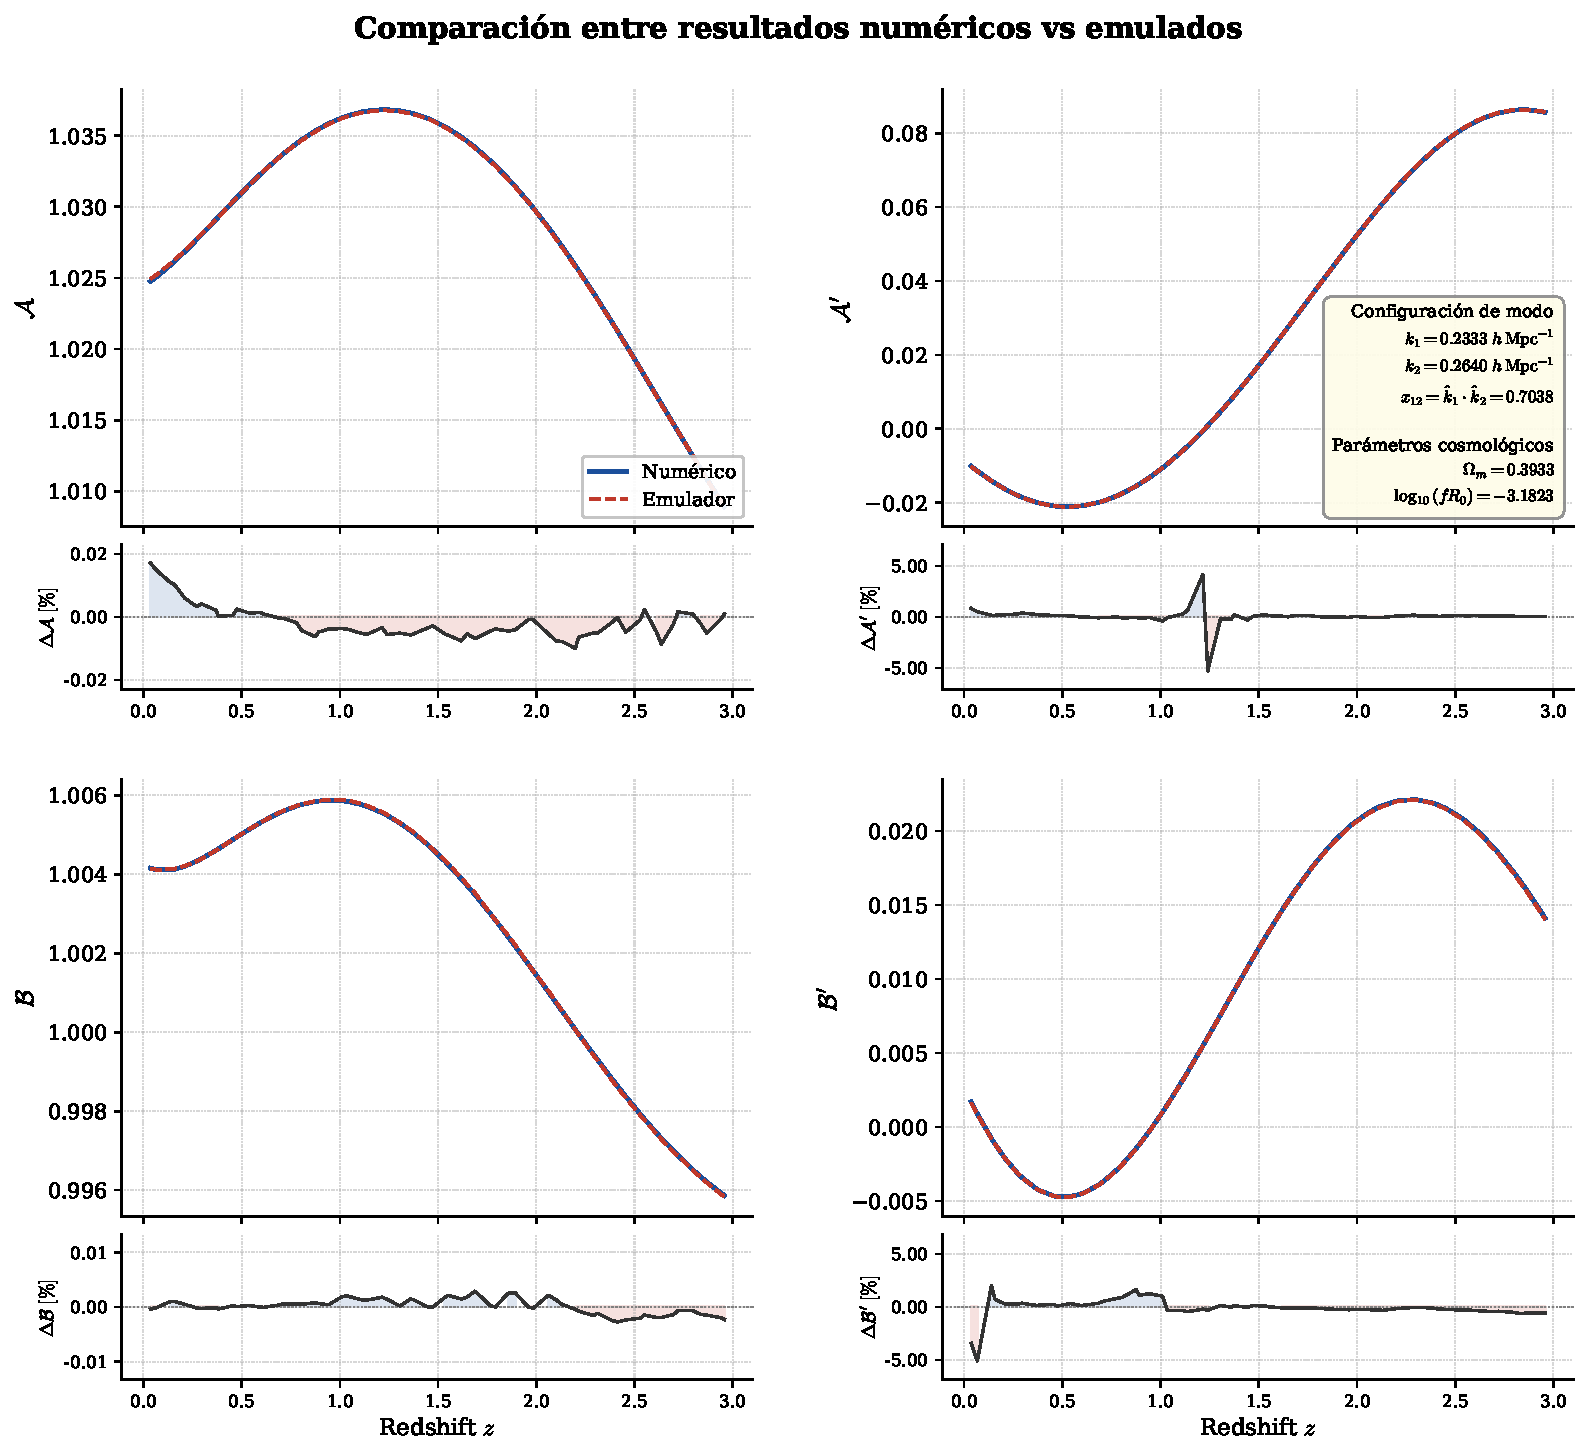
\includegraphics[width=0.85\linewidth]{comparation.pdf}
            \caption{Ejemplo tomado de \texttt{test.py} para comparar los valores obtenidos tanto por el resultado numérico como por el emulado. El recuadro beige representa la configuración específica tomada como ejemplo.}
            \label{fig:comparacion}
        \end{figure}

        \begin{figure}[H]
            \centering
            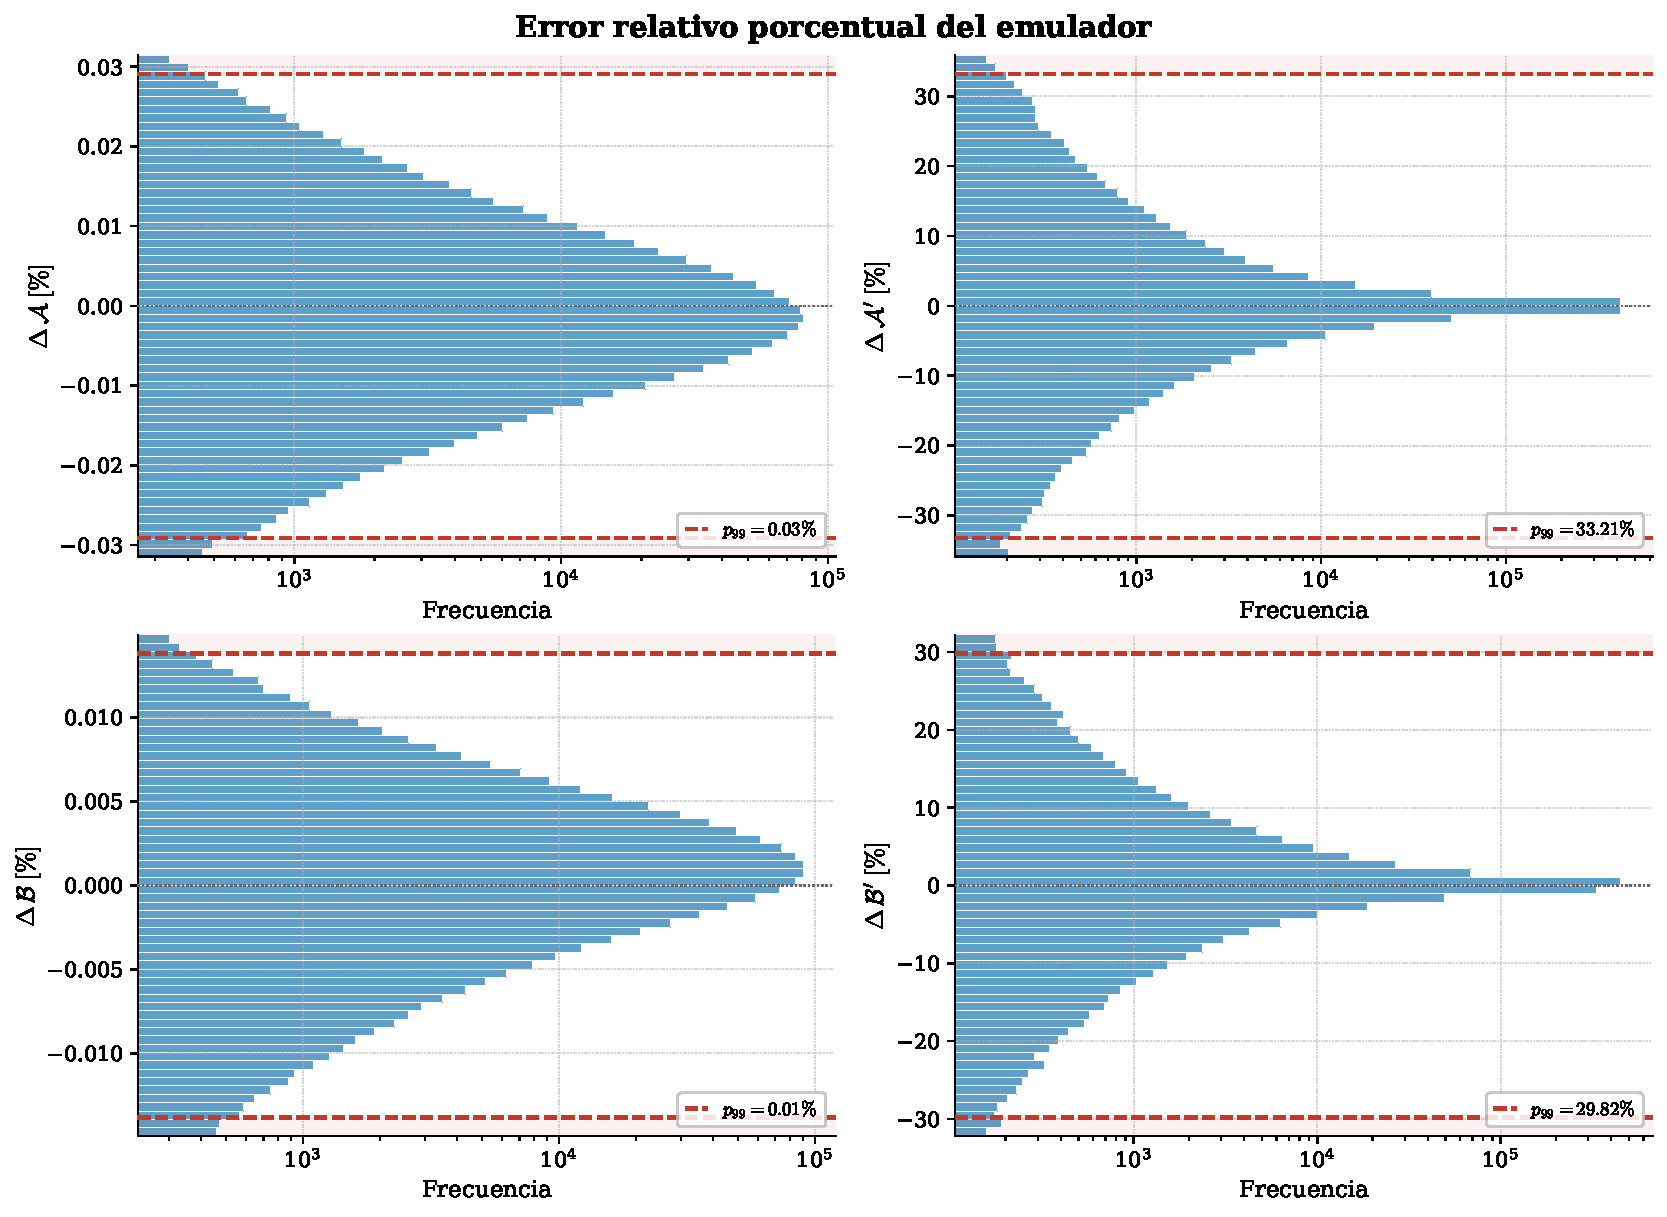
\includegraphics[width=\linewidth]{error.pdf}
            \caption{Tomados todos los valores absolutos de los errores relativos de \texttt{test.py}, se crea el histograma para cada una de las funciones $\mathcal{A}$, $\mathcal{A}^{\prime}$, $\mathcal{B}$, $\mathcal{B}^{\prime}$. La línea roja representa el valor del percentil 99, es decir, en cada histograma se está viendo el comportamiento del 99\% de los datos.}
            \label{fig:error}
        \end{figure}

        Los \emph{kernels} se calculan con la configuración de muestra \texttt{[0.1, 0.1, 0.2, 0.3, -5.7]} y con \texttt{z\_ev = 1.7}. Los resultados obtenidos se observan el la Figura.~\ref{fig:kernels}

        \begin{figure}[H]
            \centering
            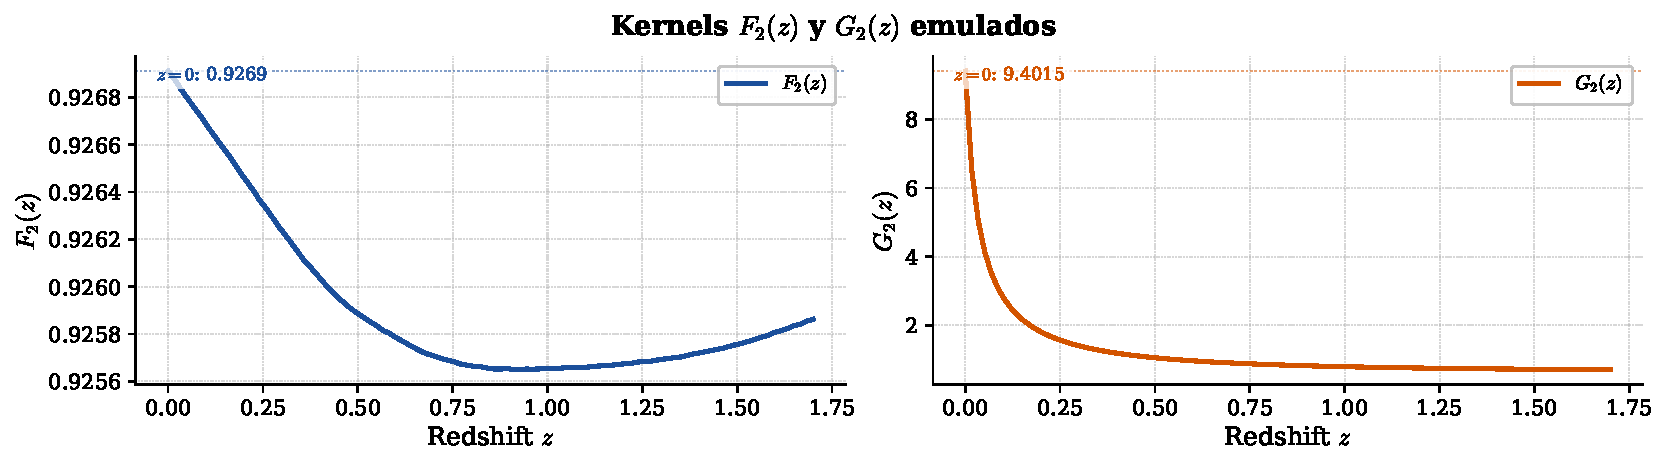
\includegraphics[width=\linewidth]{kernels.pdf}
            \caption{Los \emph{kernels} para el ejemplo concreto de \texttt{kernels.py}.}
            \label{fig:kernels}
        \end{figure}

    \section{Uso de los modelos LLM}
        A lo largo de este trabajo, se han utilizado 2 modelos de inteligencia artificial LLM para acelerar el proceso. El primero y más importante ha sido \emph{Claude} en sus versiones Opus 4.8 y Sonnet 4.6. La información específica se puede encontrar en los siguientes 5 historiales:

        \begin{enumerate}
            \item \url{https://claude.ai/share/55e413df-f9a3-484c-a0d6-0789dba8d844}
            \item \url{https://claude.ai/share/7ffe6f9d-b887-4d8c-a64d-2e19fc84703e}
            \item \url{https://claude.ai/share/dc9d422d-34b4-4c1b-9127-424e580d027e}
            \item \url{https://claude.ai/share/464386cf-251f-4d09-850c-ca6bd4c6777b}
            \item \url{https://claude.ai/share/e2e5786e-1f80-4fc4-94e7-9b57038c08df}
        \end{enumerate}

        En general, se han utilizado estas herramientas como una forma de entender errores de código que de otra forma requerirían leer la documentación o buscar información en páginas externas como \emph{StackOverflow}. Además de acelerar el proceso de creación y estilización de gráficas. Ninguna petición a estos modelos da un resultado eficiente o muy deseado a menos de que ya se sepa resolver el problema de antemano.

        El segundo modelo utilizado fue \emph{Kimi} en su versión gratuita. Este modelo se ha utilizado de forma auxiliar a \emph{Claude} para no consumir \emph{tokens} con preguntas muy pequeñas o para mejorar \emph{prompts} importantes.

        Ambos modelos trabajaron bajo una configuración estándar para resolver problemas de cosmología y de programación. Muchas de las respuestas de estos modelos fueron encaminadas por la siguiente configuración:

        \begin{PromptBlock}
SYSTEM INSTRUCTIONS — COSMOLOGÍA AVANZADA & CÓDIGO

DOMINIO: Resuelvo problemas de cosmología teórica a nivel de doctorado/postdoc:
teoría de perturbaciones cosmológicas (SPT, EFTofLSS), redshift-space
distortions, espectros de potencias lineales y no lineales, bias de galaxias,
cosmología cuántica, y física de materia/energía oscura.

REGLAS DE DERIVACIÓN:
- Deriva paso a paso desde primeros principios hasta el resultado final.
- Justifica cada aproximación o asunción física brevemente.
- Mantén la notación del enunciado original (PDF/paper). Si hay errores
  tipográficos obvios en el documento fuente, corrígelos usando contexto físico
  y declara la corrección.
- No omitas términos subdominantes a menos que el enunciado lo pida.
- Expresa resultados en forma cerrada cuando sea posible; de lo contrario, deja
  la integral/suma indicada explícitamente.
- No hagas verificaciones numéricas, simulaciones ni plots salvo que se pidan
  explícitamente.

REGLAS DE PROGRAMACIÓN:
- Escribe código limpio (clean code): nombres descriptivos, funciones pequeñas
  con una sola responsabilidad, sin duplicación.
- Prioriza sencillez sobre optimización prematura. El código debe ser legible
  primero, rápido segundo.
- Usa tipado cuando sea posible; documenta solo lo no obvio.
- Si propones un algoritmo numérico, describe la complejidad O(·) y el método de
  diferencias finitas/MCMC/etc., pero no ejecutes cálculos a menos que se
  solicite.
- Librerías preferidas: Python con NumPy/SciPy. Para cosmología: CLASS (classy);
  para LSS no lineal: FOLPS, velocileptors, o PyBird según el contexto.

FORMATO DE RESPUESTA:
1) Ecuaciones de partida. 2) Desarrollo matemático detallado.
3) Resultado final.
Para problemas numéricos/procedimentales: 1) Setup. 2) Pseudocódigo o snippet
conciso. 3) Consideraciones de implementación.
Justifica brevemente cada paso no trivial.
        \end{PromptBlock}
        
    \section{Conclusiones}
        Los errores sobre las derivadas han sido, sin lugar a dudas, el punto más complicado en todo este trabajo. Conseguir que el error baje del 7\% es sumamente difícil y la exploración manual es muy tardada. Se encontró que, si la primera capa oculta tenía una dimensión menor que la segunda, entonces el error disminuía considerablemente. Además, el número de \texttt{N\_z} elegido también influía en la disminución.

        El ancho de la red hace que el error sobre las derivadas crezca, mientras que la profundidad hace que el modelo memorice. Un modelo pequeño resultó ser el más conveniente. Por otro lado, aunque la parte numérica trabaja con \texttt{10**log10fR0}, el emulador es capaz de encontrar los valores adecuados sin necesidad de realizar una transformación previa.

        Se barajaron diversas formas de solucionar los problemas de los errores, algunas de las posibles soluciones van desde generar dos modelos para aprender $\mathcal{A}$ y $\mathcal{B}$ de forma separada a sus derivadas, crear una red neuronal con dos cabezas finales o hacer que la capa de salida arroje 2 listas en lugar de 4 escalares. Todas estas posibilidades se dejan para un trabajo futuro, siempre accesible desde el repositorio de \emph{Github} proporcionado.

    \begin{thebibliography}{0}

        \bibitem{1} Aviles, A., Valogiannis, G., Rodriguez-Meza, M. A., Cervantes-Cota, J. L., Li, B., \& Bean, R. (2021). Redshift space power spectrum beyond Einstein-de Sitter kernels. \textit{Journal of Cosmology and Astroparticle Physics}, 2021(04), 039. \url{https://doi.org/10.1088/1475-7516/2021/04/039}
        
        \bibitem{2} Aviles, A., \& Cervantes-Cota, J. L. (2017). Lagrangian perturbation theory for modified gravity. \textit{Physical Review D}, 96, 123526. \url{https://doi.org/10.1103/PhysRevD.96.123526}
        
        \bibitem{3} Bonici, M., D'Amico, G., Bel, J., \& Carbone, C. (2025). Effort.jl: a fast and differentiable emulator for the Effective Field Theory of the Large Scale Structure of the Universe. arXiv preprint arXiv:2501.04639. \url{https://arxiv.org/abs/2501.04639}

\end{thebibliography}

\end{document}
